\documentclass{article}

\usepackage[nomathjax]{bookml/bookml}
\usepackage[all]{xy}
\usepackage[pdfusetitle]{hyperref}
\usepackage{amsmath}
\usepackage{graphicx}
\usepackage{tikz}
\usetikzlibrary{cd}

\title{BookML test: images}
\author{Vincenzo Mantova}
\date{2026-09-02}

\usepackage{bookml/bookml}
\usepackage{framed}
\AtBeginDocument{\begin{framed}
  \begin{description}
    \item[BookML] \BookMLversion
    \item[\LaTeXML] \LaTeXMLversion{} (\csname bml@generator@engine\endcsname)
    \item[\LaTeX] \fmtversion
  \end{description}
\end{framed}}


\begin{document}

\section{EPS/PDF to SVG}

Samples: \includegraphics[height=3ex]{europasslogo}.%, \includegraphics[height=1.5ex]{europasslogo.eps}.

\section{BookML images}

\[ \text{straight \Xy-matrix: }
\xymatrix{
  A \ar[rd] \ar^\phi[r] & B \\
                        & C } \]
\[ \text{\Xy-matrix in \texttt{bmlimage}: }\begin{bmlimage}
\xymatrix{
  A \ar[rd] \ar^\phi[r] & B \\
                        & C }
\end{bmlimage} \]

\section{Inline SVGs}

\xymatrix{A \ar[d]^q \\ B }
$\xymatrix{
  A \ar[rd] \ar^\phi[r] & B \\
                        & C }$
\xymatrix{
A \ar@{->>}[rd] \ar@{^{(}->}[r]
&B \ar@{.>}[d]
&C \ar@{_{(}->}[l]\ar@{->>}[ld]\\
&D}

\[
\xymatrix{
T \ar@/_/[ddr]_y \ar@/^/[drr]^x \ar@{.>}[dr]|-{(x,y)}\\
&X \times_Z Y \ar[d]^q \ar[r]_p & X\ar[d]_f \\
&Y \ar[r]^g &Z}
\]

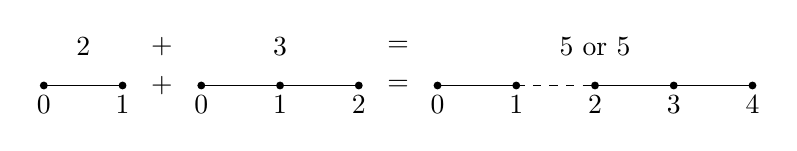
\begin{tikzpicture}
  \draw (0.5,0.5) node {$2$};
  \draw (1.5,0.5) node {$+$};
  \draw (3,0.5) node {$3$};
  \draw (4.5,0.5) node {$=$};
  \draw (7,0.5) node {$5$ or $5$};
  \draw (0,0) node [below] {$0$} -- (1,0) node [below] {$1$};
  \draw (1.5,0) node {$+$};
  \draw (2,0) node [below] {$0$} -- (3,0) node [below] {$1$} -- (4,0) node [below] {$2$};
  \draw (4.5,0) node {$=$};
  \draw (5,0) node [below] {$0$} -- (6,0) node [below] {$1$};
  \draw [dashed] (6,0) -- (7,0);
  \draw (7,0) node [below] {$2$} -- (8,0) node [below] {$3$} -- (9,0) node [below] {$4$};
  \foreach \x in {0,1,2,3,4,5,6,7,8,9} {
      \fill (\x,0) circle (0.05);
    }
\end{tikzpicture}
\begin{tikzcd}
A \arrow[r, "\phi"] \arrow[d, red]
& B \arrow[d, "\psi" red] \\
C \arrow[r, red, "\eta" blue]
& |[blue, rotate=-15]| D
\end{tikzcd}
\begin{tikzcd}
  A \arrow[r, "\phi\eta" near start, "\phi" near start, "\psi"',"\normalsize \eta x_i^2" near end] & {\hbox{\large B}}
\end{tikzcd}
\begin{tikz}
  \node[rectangle, draw] {\vbox{Line 1.

  Line 2, longer.}};
\end{tikz}

\end{document}
